\documentclass[10pt,unicode, notheorems]{beamer}

\usetheme[numbers, totalnumbers,minimal]{Statmod}
\usepackage[T2A]{fontenc}
\usepackage[utf8]{inputenc}
\usepackage[russian]{babel}
\usepackage{amsthm}
\usepackage{amsmath}
\usepackage{bm}
\usepackage{bbold}
\newtheorem{result}{Утверждение}
\newtheorem{theorem}{Теорема}
\newtheorem{remark}{Предложение}
\newtheorem{theorem+}{Теорема Гаусса-Маркова}
\newtheorem{theoremCT}{Теорема Куна-Таккера}
\DeclareMathOperator{\E}{E} 
\DeclareMathOperator{\T}{T} 
\DeclareMathOperator{\D}{D} 

\title{Обучение с учителем. Регрессия. Регуляризация}
\author[Е. Романова, А. Горбачук, Д. Сидоренко]{Романова Елизавета, Горбачук Анна, Сидоренко Денис}
\institute[СПбГУ]{Санкт-Петербургский государственный университет \\
    Прикладная математика и информатика \\
    Кафедра статистического моделирования\\ 
}
\date{
    Санкт-Петербург\\
    2019г.
}
\begin{document}
\begin{frame}
    \titlepage
\end{frame}

\begin{frame}
\frametitle{Введение}
\framesubtitle{Обучение с учителем}

\begin{itemize}
\item $Y$ --- количественный отклик, $X_{1},\ldots,X_{p}$ --- предикторы, $X=(X_{1},\ldots,X_{p})$.
\item Предполагаем существование зависимости $Y=f^{\ast}(X)+\varepsilon$.
\item $\varepsilon$ --- ошибка, которая не зависит от $X$, $\mathrm{E}\varepsilon=0$.
\item $x_{1},\ldots,x_{n}$ --- наблюдения, $x_{i}=(x_{i1},\ldots,x_{ip})^{\mathrm{T}}$, $y_{i}$ --- отклик $i$-го наблюдения.
\item $(x_{i},y_{i})_{i=1}^{n}$ --- обучающая выборка, участвует в оценке $f^{\ast}$.
\item $(x_{i}^{\prime},y_{i}^{\prime})_{i=1}^{k}$ --- тестовая выборка, не участвует в оценке $f^{\ast}$.
\item Задача: найти такую функцию $\hat{f}$, что $y\approx\hat{f}(x)$ для любого наблюдения $(x,y)$.
\end{itemize}
\end{frame}


\begin{frame}
\frametitle{Регрессия}

\begin{itemize}
\item $X_{n}=(x_{i},y_{i})_{i=1}^{n}$ --- обучающая выборка, $x_{i}\in\mathbb{R}^{p}$, $y_{i}\in\mathbb{R}$.
\item $y_{i}=f^{\ast}(x_{i})+\varepsilon_{i}$, $i=1,\ldots,n$.
\item Модель регрессии: параметрическое семейство функций $f(x,\theta)$, где $\theta\in\Theta\subset\mathbb{R}^{p}$ --- вектор параметров модели.
\item Средняя квадратичная ошибка (функционал качества, наиболее часто применяющийся в задачах регрессии):
\begin{equation*}
Q(\theta,X_{n})=
\sum_{i=1}^{n}
(f(x_{i},\theta)-y_{i})^{2}.
\end{equation*}
\item Задача обучения по МНК --- задача минимизации
\begin{equation*}
Q(\theta,X_{n})
\rightarrow
\min_{\theta\in\Theta}.
\end{equation*}
\end{itemize}
\end{frame}

\begin{frame}
\frametitle{Проблема}
\begin{itemize}
\item Минимизируем среднюю квадратичную ошибку на обучающей выборке:
\begin{equation*}
\mathrm{MSE}_{\text{train}}
=
\frac{1}{n}Q(B,X)
\rightarrow
\min.
\end{equation*}
\item Истинная цель --- минимизировать ошибку на всем пространстве объектов, то есть минимизировать $\mathrm{MSE_{\text{test}}}=Q(X^{\prime},B)/k$, где  $X^{\prime}=(x_{i}^{\prime},y_{i}^{\prime})_{i=1}^{k}$ --- произвольная контрольная выборка.
\item Нет гарантии, что оптимальные для $\mathrm{MSE}_{\text{train}}$ параметры будут минимизировать  $\mathrm{MSE_{\text{test}}}$.
\item Может возникнуть переобучение (переподгонка): $\mathrm{MSE_{\text{test}}}\gg\mathrm{MSE}_{\text{train}}$.
\end{itemize}
\end{frame}


\begin{frame}
\frametitle{Bias–variance tradeoff}

 Пусть $(x^{\prime},y^{\prime})\in X_{k}^{\prime}$ --- объект данных из тестовой выборки, $y^{\prime}=f^{\ast}(x^{\prime})+\varepsilon$, $\E\varepsilon=0$, $\E\varepsilon^{2}=\sigma^{2}$. 
 
Для математического ожидания квадрата ошибки предсказания на $(x^{\prime},y^{\prime})$ справедливо
\begin{equation*}
\E(\hat{f}(x^{\prime})-y^{\prime})^{2}
=
\D\hat{f}(x^{\prime})+(\mathrm{Bias}\hat{f}(x^{\prime}))^{2}+\sigma^{2},
\end{equation*}
$\D\hat{f}$ --- дисперсия оценки $\hat{f}$, $\mathrm{Bias}\hat{f}(x^{\prime})$ --- смещение оценки, $\sigma^{2}$ --- неустранимая ошибка.

\begin{itemize}
\item $\mathrm{MSE}$ на контрольной выборке зависит от дисперсии оценки и квадрата ее смещения.\\
\item Дисперсия оценки определяет, насколько изменится $\hat{f}$, если бы мы получали эту оценку по другому набору данных. 
\item Смещение $\hat{f}$ характеризует ошибку, возникающую при аппроксимации сложной функции $f^{\ast}$ более простой моделью.
\item Нужен метод обучения, который обеспечивает и низкую дисперсию, и низкое смещение.
\end{itemize}
\end{frame}

\begin{frame}
\frametitle{Множественная линейная регрессия}
\begin{itemize}
\item Пусть зависимость между ответами и признаками линейна. 
\item Пусть ответы и признаки центрированы.
\item Модель множественной линейной регрессии:
\begin{equation*}
y_{i}
=
f(x_{i},B)+\varepsilon_{i}
=
\sum_{j=1}^{p}\beta_{j}x_{ij}+\varepsilon_{i}.
\end{equation*}
\item 
Задача -- минимизировать функционал качества:
\begin{equation*}
Q(B,X)
=
\sum_{i=1}^{n}
\left(
y_{i}-
\sum_{j=1}^{p}\beta_{j}x_{ij}
\right)^{2}
\rightarrow
\min_{\beta_{1},\ldots,\beta_{p}}.
\end{equation*}
\end{itemize}
\end{frame}


\begin{frame}
\frametitle{Множественная линейная регрессия}
\framesubtitle{Задача оптимизации}

Введем матричные обозначения:
\begin{itemize}
\item  $\mathbb{X} = [X_1, \ldots, X_p]$, где $X_i = (x_{1i}, \ldots, x_{ni})^{\T}$, $i = 1, \ldots, p$,
\item  $Y=(y_{1},\ldots,y_{n})^{\mathrm{T}}$, $\mathcal{E}=(\varepsilon_{1},\ldots,\varepsilon_{n})^{\mathrm{T}}$, 
\item  $B=(\beta_{1},\ldots,\beta_{p})$ --- вектор параметров модели.
\end{itemize}

Модель линейной регрессии в матричной форме:
\begin{equation*}
Y=\beta_{1}X_{1}+\cdots+\beta_{p}X_{p}+\mathcal{E}
=
\mathbb{X}B+\mathcal{E}.
\end{equation*}

Задача оптимизации принимает вид: 
\begin{equation*}
Q(B,X)=
||Y-\mathbb{X}B||^{2}
\rightarrow
\min_{B}.
\end{equation*}

Решение МНК: $\hat{B}=(\mathbb{X}^{\mathrm{T}}\mathbb{X})^{-1}\mathbb{X}^{\mathrm{T}}Y=\mathbb{X}^{-}Y$, 
$\hat{Y}=\mathbb{X}\hat{B}$.

\end{frame}

\begin{frame}
\frametitle{Множественная линейная регрессия}
\framesubtitle{МНК-решение}

Решение МНК: $\hat{B}=(\mathbb{X}^{\mathrm{T}}\mathbb{X})^{-1}\mathbb{X}^{\mathrm{T}}Y=\mathbb{X}^{-}Y$, 
$\hat{Y}=\mathbb{X}\hat{B}$.

При плохой обусловленности матрицы вычисление обратной матрицы крайне нежелательно. Варианты обхода:
\begin{itemize}
\item Решать соответствующую нормальную систему (например, при помощи QR-разложения)
\begin{equation*}
\mathbb{X}^{\mathrm{T}}Y=
\mathbb{X}^{\mathrm{T}}\mathbb{X}B.
\end{equation*}
\item Использовать SVD.
Пусть $\mathbb{X}=\mathbb{V}\mathbb{\Lambda}\mathbb{U^{\mathrm{T}}}$ --- сингулярное разложение $\mathbb{X}$.
 Тогда вектор МНК-решения легко записать в виде
\begin{equation*}
\hat{B}=\mathbb{X}^{-}Y
=
\sum_{j=1}^{p}
\frac{1}{\sqrt{\lambda_{j}}}
U_{j}(V_{j}^{\mathrm{T}}Y).
\end{equation*}
\end{itemize}
\end{frame}

\begin{frame}
\frametitle{Множественная линейная регрессия}
\framesubtitle{Сингулярное разложение}
Пусть $\mathbb{X}=\mathbb{V}\mathbb{\Lambda}\mathbb{U^{\mathrm{T}}}$ --- сингулярное разложение $\mathbb{X}$.
\begin{itemize}
\item Тогда псевдообратную к $\mathbb{X}$ матрицу легко записать в виде
\begin{equation*}
\mathbb{X}^{-}
=
\mathbb{U}\mathbb{\Lambda}^{-1}\mathbb{V}^{\mathrm{T}}
=
\sum_{j=1}^{p}
\frac{1}{\sqrt{\lambda_{j}}}
U_{j}V_{j}^{\mathrm{T}}.
\end{equation*}
\item Вектор МНК-решения:
\begin{equation*}
\hat{B}=\mathbb{X}^{-}Y
=
\sum_{j=1}^{p}
\frac{1}{\sqrt{\lambda_{j}}}
U_{j}(V_{j}^{\mathrm{T}}Y).
\end{equation*}
\item  Оценка вектора $Y$:
\begin{equation*}
\hat{Y}
=
\mathbb{X}\hat{B}
=
\sum_{j=1}^{p}
V_{j}(V_{j}^{\mathrm{T}}Y).
\end{equation*}
\item Норма вектора коэффициентов:
\begin{equation*}
||\hat{B}||^{2}
=
\sum_{j=1}^{p}
\frac{1}{\lambda_{j}}(V_{j}^{\mathrm{T}}Y)^{2}.
\end{equation*}
\end{itemize}
\end{frame}




\begin{frame}
\frametitle{Мультиколлинеарность признаков}
\textbf{Избыточность.}

Рассмотрим случай, когда матрица данных содержит несколько сильно коррелированных признаков (есть $\lambda_{j}\rightarrow0$). Что будет происходить в таком случае с МНК-оценкой:
\begin{itemize}
\item Решение $\hat{B}$  неустойчиво, 
\item Решение неинтерпретируемо,  $||\hat{B}||\rightarrow\infty$,
\item Ответы на контрольной выборке неустойчивы,
\item На обучающей выборке все хорошо:
\begin{equation*}
||\mathbb{X}\hat{B}-Y||^{2}
\rightarrow0.
\end{equation*}
\end{itemize}
\textbf{Способы решения проблемы:}
\begin{itemize}
\item Отбор признаков.
\item Преобразование признаков.
\item Регуляризация.
\end{itemize}
\end{frame}


\begin{frame}
\frametitle{Регуляризация}

\begin{itemize}
\item  $\mathrm{MSE}_{\mathrm{test}}$ зависит от дисперсии оценки $\hat{f}$ и ее смещения.
\item Когда связь между откликом и предикторами (почти) линейна, оценки по МНК обладают (почти) нулевым смещением, но при этом могут иметь большую дисперсию. 
\item Ковариационная матрица МНК-оценки $\hat{B}$: 
\begin{equation*}
\mathrm{Cov}(\hat{B}) = \sigma^2(\mathbb{X}^{\T}\mathbb{X})^{-1}.
\end{equation*}
\item Чем больше дисперсия оценки $\hat{B}$, тем больше дисперсия $\hat{f}$. 
\item Когда матрица $\mathbb{X}$ близка к вырожденной, дисперсия $\hat{B}$ становится большой и $\mathrm{MSE}_{\mathrm{test}}$ увеличивается.  
\item При $p>n$ или при полностью коллинеарных признаках оценки по МНК не имеют уникального решения.
\item Введение небольшого смещения в оценке может привести к уменьшению дисперсии и тем самым уменьшению $\mathrm{MSE}_{\text{test}}$.
\end{itemize}

\end{frame}


\begin{frame}
\frametitle{Регуляризация Тихонова}

\begin{itemize}
\item МНК решает нормальную систему $\mathbb{X}^{\T}\mathbb{X}B=\mathbb{X}^{\T}Y$.
\item При наличии сильно скоррелированных признаков матрица $\mathbb{X}^{\T}\mathbb{X}$  близка к вырожденной.
\item \textbf{Регуляризация Тихонова}: прибавляем к матрице $\mathbb{X}^{\T}\mathbb{X}$ матрицу $\mathbb{T}^{\T}\mathbb{T}$ так, чтобы их сумма была хорошо обусловлена.
\item Переходим к нормальной системе $(\mathbb{X}^{\T}\mathbb{X}+\mathbb{T}^{\T}\mathbb{T})B=\mathbb{X}^{\T}Y$.
\item Решение системы соответствует минимизации функции 
\begin{equation*}
||Y-\mathbb{X}B||_{2}^{2}+||\mathbb{T}B||_{2}^{2}.
\end{equation*}
\item Решение:  
$
\hat{B}_{T}
=(\mathbb{X}^{\T}\mathbb{X}+\mathbb{T}^{\T}\mathbb{T})^{-1}\mathbb{X}^{\T} Y
$.
\item 
$
\E\hat{B}_{T}
=
(\mathbb{X}^{\T}\mathbb{X}+\mathbb{T}^{\T}\mathbb{T})^{-1}\mathbb{X}^{\T}\mathbb{X}B
$.
\item
$
\mathrm{Cov}(\hat{B}_{T})
=
\sigma^{2}
(\mathbb{X}^{\T}\mathbb{X}+\mathbb{T}^{\T}\mathbb{T})^{-1}
\mathbb{X}^{\T}\mathbb{X}
((\mathbb{X}^{\T}\mathbb{X}+\mathbb{T}^{\T}\mathbb{T})^{-1})^{\T}
$.
\end{itemize}
\end{frame}

\begin{frame}
\frametitle{Гребневая регрессия (Ridge regression)}


\begin{itemize}
\item Гребневая регрессия --- это частный случай регуляризации Тихонова с $\mathbb{T}=\sqrt{\tau}\mathbb{I}$.
\item Вводим штраф за увеличение нормы вектора $B$ и переходим к минимизации следующей функции:
\begin{equation*}
Q_{\tau}(B)
=
||\mathbb{X}B-Y||^{2}
+
\tau||B||^{2}
\rightarrow\min_{B},
\end{equation*}
где $\tau$ --- неотрицательный параметр регуляризации.
\item В развернутом виде задача оптимизации записывается так:
\begin{equation*}
\sum_{i=1}^{n}
\left(
y_{i}
-
\sum_{j=1}^{p}\beta_{j}x_{ij}
\right)^{2}
+
\tau\sum_{j=1}^{p}\beta_{j}^{2}
\rightarrow\min_{B}.
\end{equation*}
\item Решение:
\begin{equation*}
\hat{B}_{\tau}
=
(\mathbb{X}^{\mathrm{T}}\mathbb{X}+\tau\mathbb{I}_{p})^{-1}\mathbb{X}^{\mathrm{T}}Y.
\end{equation*}
\end{itemize}

\end{frame}



\begin{frame}
\frametitle{Гребневая регрессия (Ridge regression)}
\framesubtitle{Параметр регуляризации}
Задача гребневой регрессии:
\begin{equation*}
\sum_{i=1}^{n}
\left(
y_{i}
-
\sum_{j=1}^{p}\beta_{j}x_{ij}
\right)^{2}
+
\tau\sum_{j=1}^{p}\beta_{j}^{2}
\rightarrow\min_{B}.
\end{equation*}
\begin{itemize}
\item $\tau\sum_{j = 1}^p \beta_j^2$ мало, когда $\beta_1, \ldots, \beta_p$ близки к нулю.
\item Чем больше коэффициент регуляризации $\tau$, тем устойчивее решение, но больше смещение.
\item Когда $\tau = 0$, то гребневая регрессия совпадает с обычной регрессией, но при $\tau \rightarrow \infty$ коэффициенты регрессии стремятся к нулю.
\item Необходимо выбрать хорошее ("Компромиссное") значение $\tau$.
\end{itemize}
\end{frame}



\begin{frame}
\frametitle{Гребневая регрессия (Ridge regression)}
\framesubtitle{Параметр регуляризации}
 
 \begin{itemize}
 \item  Решение задачи гребневой регрессии:
\begin{equation*}
\hat{B}_{\tau}
=
(\mathbb{X}^{\mathrm{T}}\mathbb{X}+\tau\mathbb{I}_{p})^{-1}\mathbb{X}^{\mathrm{T}}Y.
\end{equation*}
 \item Подход на основе сингулярного разложения $\mathbb{X}=\mathbb{V}\mathbb{\Lambda}\mathbb{U^{\mathrm{T}}}$ позволяет подбирать параметр $\tau$, вычислив SVD только один раз.
 \item Решение гребневой регрессии через SVD:
\begin{equation*}
\hat{B}_{\tau} = \mathbb{U}(\mathbb{\Lambda}^2 +\tau \mathbb{I}_{p})^{-1}\mathbb{\Lambda}\mathbb{V}^{\T}Y 
= \sum_{j=1}^p \frac{\sqrt{\lambda_j}}{\lambda_j + \tau} U_j(V_j^{\T}Y).
\end{equation*}
 \item Оценка функции $f^{\ast}$ для выборки $X$ через SVD:
\begin{equation*}
\mathbb{X}\hat{B}_{\tau} = \mathbb{V}\mathbb{\Lambda}\mathbb{U}^{\T}\hat{B}_{\tau} = \mathbb{V} \mathrm{diag}(\frac{\lambda_j}{\lambda_j + \tau})\mathbb{V}^{\T}Y = \sum_{j=1}^p \frac{\lambda_j}{\lambda_j + \tau} V_j(V_j^{\T}Y).
\end{equation*}
 \end{itemize}

\end{frame}


\begin{frame}
\frametitle{Подбор параметра $\tau$ }

\textbf{Скользящий контроль}:%см слайд 41 в 08 короба
\begin{itemize}
\item выбираем сетку значений $\tau$;
\item вычисляем ошибку кросс-проверки для каждого значения $\tau$;
\item выбираем $\tau$ с наименьшим значением ошибки кросс-проверки;
\item перестраиваем модель со всеми наблюдениями с выбранным значением $\tau$.
\end{itemize}

\textbf{Эвристика }(практические рекомендации, Воронцов К. В.):
\begin{itemize}
\item брать $\tau$ в отрезке $[0.1, 0.4]$, если столбцы матрицы $\mathbb{X}$ заранее
стандартизованы.
\item выбрать $\tau$ так, чтобы число обусловленности матрицы $\mathbb{X}^{\mathrm{T}}\mathbb{X}+\tau\mathbb{I}_{p}$ приняло заданное не слишком большое значение $M_{0}$, откуда следует рекомендация $\tau\approx\lambda_{max}/M_{0}$.
\end{itemize}
\end{frame}





\begin{frame}
\frametitle{Вероятностная интерпретация гребневой регрессии}
\begin{itemize}
\item Модель: $Y=\mathbb{X}B+\mathcal{E}$.
\item Ошибки независимы и $\varepsilon_{i}\in N(0,\sigma^{2})$.
\item Пусть выборка $(x_{i},y_{i})_{i=1}^{n}$ из распределения с плотностью $p$.
\item Функция правдоподобия выборки (совместное распределение независимой выборки): $L(X,Y,B)=\prod_{i=1}^{n}p(x_{i},y_{i},B)$.
\item Пусть вектор параметров $B$ имеет априорное распределение $\pi(B)$.
\item По теореме Байеса при фиксированном $X$ апостериорное распределение $q(B|X,Y)$ пропорционально $L(X,Y,B)\pi(B)$.
\item Если $\pi(B)\stackrel{d}{=}N(\bm{0},\frac{\sigma^{2}}{\tau}\mathbb{I})$, то оценка апостериорного максимума $B$ совпадает с решением гребневой регрессии.
\end{itemize}
\end{frame}

\begin{frame}
\frametitle{Выкладки}
Оценка максимума апостериорной вероятности:
\begin{multline*}
\arg\max_{\beta_{1},\ldots,\beta_{p}}\exp
\left(
-\sum_{j=1}^{n}
\frac{\varepsilon_{j}^{2}}{2\sigma^{2}}
\right)
\exp\left(
-\sum_{i=1}^{p}
\frac{\tau\beta_{i}^{2}}{2\sigma^{2}}\right)
=\\=
\arg\max_{\beta_{1},\ldots,\beta_{p}}\exp
\left(-\sum_{j=1}^{n}
\frac{(y_{j}-\sum_{i=1}^{p}\beta_{i}x_{ij})^{2}}{\sigma^{2}}
\right)
\exp
\exp\left(
-\sum_{i=1}^{p}
\frac{\tau\beta_{i}^{2}}{2\sigma^{2}}\right)
=\\=
\arg\max_{B}
\exp
\left(
-\frac{||Y-\mathbb{X}B||^{2}}{2\sigma^{2}}-\frac{\tau||B||^{2}}{2\sigma^{2}}
\right)
=\\=
\arg\min_{B}
(||Y-\mathbb{X}B||^{2}+\tau||B||^{2}).
\end{multline*}

Пришли к решению задачи гребневой регрессией с параметром регуляризации $\tau$.
\end{frame}

\begin{frame}
\frametitle{Гребневая регрессия (Ridge regression)}
\framesubtitle{Свойства}
\begin{itemize}
\item Стандартные МНК-оценки инварианты относительно умножения признака на константу, то есть значение $X_{j}\hat{\beta_j}$ не зависит от масштаба $j$-го признака. 
\item Оценки МНК гребневой регрессии не обладают свойством инвариантности и могут существенно меняться.
\end{itemize}

\vspace{0.3cm}
\textbf{Вывод:} гребневую регрессию нужно использовать после стандартизации признаков.
\vspace{0.8cm}

\textbf{Проблемы:} 
\begin{itemize}
\item в конечную модель входят все начальные признаки;
\item если признаков много, то усложняется интерпретация.
\end{itemize}

\end{frame}

\begin{frame}
\frametitle{Лассо регрессия}
%С этими недостатками справляется Лассо рергессия, в которой в качестве штрафа используется $l_{1}$-норма вектора коэффициентов
\begin{itemize}
\item Рассмотрим метод, в котором в качестве штрафа за увеличение нормы вектора $B$ используется его $l_{1}$-норма.
\item Метод LASSO решает следующую задачу минимизации:
\begin{equation*}
||\mathbb{X}B-Y||_{2}^{2}
+
\tau||B||_{1}^{2}
\rightarrow\min_{B},
\end{equation*}
где $\tau$ --- неотрицательный параметр регуляризации.
\item Задача оптимизации в развернутом виде:
\begin{equation*}
\sum_{i=1}^{n}
\left(
y_{i}
-
\sum_{j=1}^{p}\beta_{j}x_{ij}
\right)^{2}
+
\tau\sum_{j=1}^{p}|\beta_{j}|
\rightarrow\min_{\beta_{1},\ldots,\beta_{p}}.
\end{equation*}
\item Хотим применить теорему Куна-Таккера.
\item Проблема: целевая функция не гладкая. 
\end{itemize}
\end{frame}




\begin{frame}
\frametitle{Теорема Куна-Таккера}

Пусть $x\in\mathbb{R}^{n}$. Рассмотрим задачу 
\begin{gather*}
f(x)\to\min,\\
g_{i}(x)\leq 0,
\quad
i=0,\ldots,m.
\end{gather*}

Функция Лагранжа:
\begin{equation*}
\mathcal{L}(x;\mu,\lambda)
=
f(x)+
\sum_{i=1}^{m}\lambda_{i}g_{i}(x).
\end{equation*}

\begin{theoremCT}
Пусть $f(x)$ выпукла и дифференцируема на допустимом множестве. Все ограничения регулярные (аффинные функции).
Тогда $x_{\ast}$ --- оптимальное решение, тогда и только тогда, когда $\exists,\lambda_{i}$ такие, что 
\begin{gather*}
\frac{\partial f(x_{\ast})}{\partial x_{j}}
+
\sum_{i=1}^{m}\lambda_{i}\frac{\partial g(x_{\ast})}{\partial x_{j}}=0
\quad
j=1,\ldots,n,\\
g_{i}(x_{\ast})\leq 0,\quad
\lambda_{i}\geq 0,
\quad
\lambda_{i}g_{i}(x_{\ast})=0,
\quad
i=1,\ldots,m.
\end{gather*}
\end{theoremCT}

\end{frame}

\begin{frame}
\frametitle{Решение задачи оптимизации}
\begin{itemize}
\item Задачу lasso-оптимизации можно переписать в форме с ограничениями: %(метод множителей Лагранжа):
\begin{equation*}
\begin{cases}
\sum_{i=1}^{n}
\left(
y_{i}
-
\sum_{j=1}^{p}\beta_{j}x_{ij}
\right)^{2}
\to
\min_{\beta_{1},\ldots,\beta_{p}},\\
\sum_{j=1}^{p}|\beta_{j}|\leq\ae,
\end{cases}
\end{equation*}
где $\ae=1/\tau$.
\item После замены $\beta_{j}=\beta_{j}^{+}-\beta_{j}^{-}$, $|\beta_{j}|=\beta_{j}^{+}+\beta_{j}^{-}$, переходим к задаче оптимизации ($2p$ переменных, $2p+1$ ограничений):
\begin{equation*}
\begin{cases}
\sum_{i=1}^{n}
\left(
y_{i}
-
\sum_{j=1}^{p}(\beta_{j}^{+}-\beta_{j}^{-})x_{ij}
\right)^{2}
\to
\min_{\beta_{1}^{+},\ldots,\beta_{p}^{+},\beta_{1}^{-},\ldots,\beta_{p}^{-}},\\
\sum_{j=1}^{p}\beta_{j}^{+}+\beta_{j}^{-}\leq\ae,
\quad
\beta_{j}^{+}\geq 0,
\quad
\beta_{j}^{-}\geq 0.
\end{cases}
\end{equation*}
\item Выпуклая задача квадратичного программирования с линейными ограничениями-неравенствами.
\item Чем меньше $\ae$, тем больше $j$ таких, что  $\beta_{j}^{+}=\beta_{j}^{-}=0$.
\end{itemize}
\end{frame}



\begin{frame}
\frametitle{Вероятностная интерпретация Лассо}

\begin{itemize}
\item Модель: $Y=\mathbb{X}B+\mathcal{E}$.
\item Ошибки независимы и $\varepsilon_{i}\in N(0,\sigma^{2})$.
\item Пусть выборка $(x_{i},y_{i})_{i=1}^{n}$ из распределения с плотностью $p$.
\item Функция правдоподобия выборки (совместное распределение независимой выборки): $L(X,Y,B)=\prod_{i=1}^{n}p(x_{i},y_{i},B)$.
\item Пусть вектор параметров $B$ имеет априорное распределение $\pi(B)$.
\item По теореме Байеса при фиксированном $X$ апостериорное распределение $q(B|X,Y)$ пропорционально $L(X,Y,B)\pi(B)$.
\item Если $\pi(B)=\prod_{j=1}^{p}g(\beta_{j})$, где $g$ --- плотность распределения Лапласа $\mathrm{Laplace}(0,\tau)$, то оценка апостериорного максимума $B$ совпадает с решением лассо регрессии.
\end{itemize}
\end{frame} 




\begin{frame}
\frametitle{Сравнение гребневой регрессии и Лассо}
\begin{figure}
\center{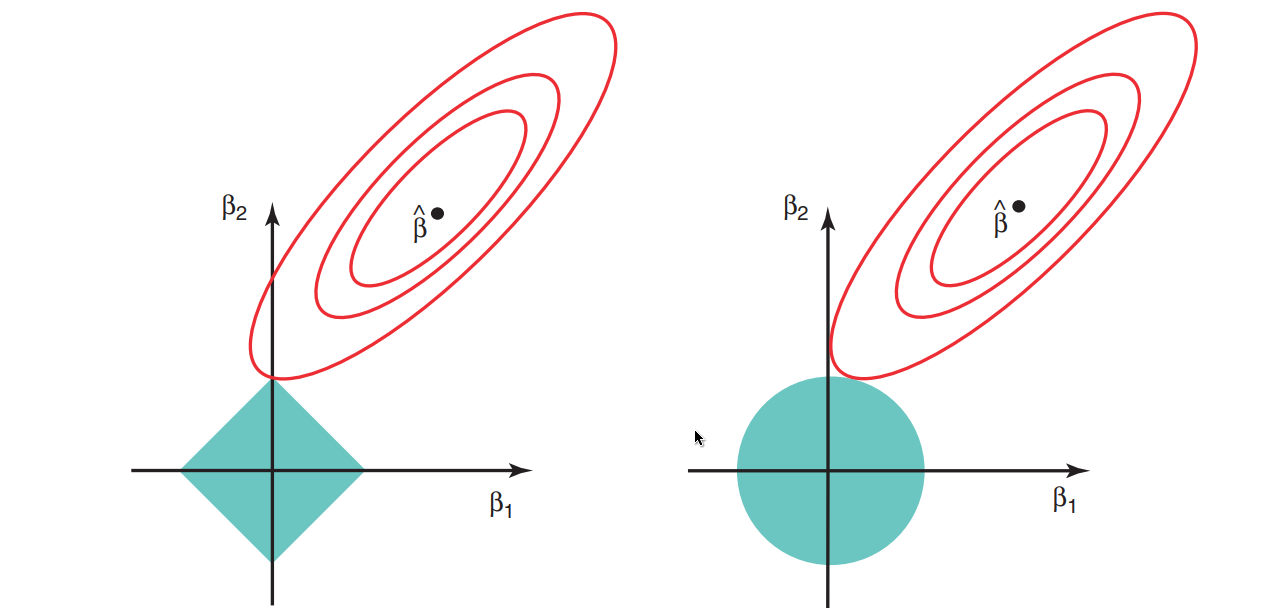
\includegraphics[width=1\linewidth]{Lasso_and_ridge.png}}
\caption{Линии уровня квадратичной функции $\sum_{i=1}^n(y_i - \sum_{j=1}^p \beta_j x_{ij})^2$ и границы ограничений для Лассо (слева) и  гребневой регрессии (справа) при $p=2$.}
\end{figure}
\end{frame}

\begin{frame}
\frametitle{Сравнение гребневой регрессии и Лассо}

\vspace{0.8cm}
\begin{itemize}
\item Обычно Лассо подходит лучше в случае наличия большого количества лишних (незначимых) признаков, 
\item Для реальных данных обычно заранее не известно количество признаков, значимо влияющих на зависимую переменную,
\item С помощью кросс-валидации можно определить какой подход лучше для конкретных данных.
\end{itemize}
\end{frame}


\begin{frame}
\frametitle{Elastic net regularization}
Решается задача оптимизации
\begin{equation*}
||Y-\mathbb{X}B||_{2}^{2} + \tau_{1}||B||_{1}^{2}+\tau_{2}||B||_{2}^{2}
\rightarrow\min_{B}.
\end{equation*}
\begin{itemize}
\item[\checkmark] Elastic net --- это комбинация методов Lasso и Ridge:
\begin{itemize}
\item Когда $\tau_1 = 0$: Ridge регрессия;
\item Когда $\tau_2 = 0$: Lasso регрессия;
\end{itemize}
\item[\checkmark] Elastic net в целом лучше, чем Lasso при наличии коррелированных признаков;
\item[\checkmark] В отличие от Ridge регрессии, когда $p > n$, Elastic net может учитывать более $n$ переменных;
\item[\checkmark] При наличии группы релевантных и избыточных признаков Lasso обычно имеет тенденцию отказываться от всех, кроме одного признака из этой группы, в то время как Elastic net будет выбирать всю группу признаков.
\item[\checkmark] Elastic net можно свести к SVM, для которого разработано много быстрых решений.
\end{itemize}
\end{frame}

\begin{frame}
\frametitle{Нелинейная регрессия}

 Нелинейная модель регрессии $f(x,\theta)$, $\theta\in\mathbb{R}^{k}$.
 Решаем задачу минимизации функционала среднеквадратичного отклонения:
\begin{equation*}
Q(\theta,X)
=
\sum_{i=1}^{n}\left(
f(x_{i},\theta)-y_{i}
\right)^{2}
\end{equation*}

\textbf{
Метод Ньютона-Рафсона:}
\begin{itemize}
\item Начальное приближение: $\theta^{0}=(\theta_{1}^{0},\ldots,\theta_{k}^{0})$,
\item Итерационный процесс: 
\begin{equation*}
\theta^{t+1}:=
\theta^{t}
-
h_{t}(Q^{\prime\prime}(\theta^{t}))^{-1}Q^{\prime}(\theta^{t}),
\end{equation*}
$Q^{\prime}(\theta^{t})$ --- градиент, $Q^{\prime\prime}(\theta^{t})$ --- гессиан, $h_{t}$ --- величина шага (простейший вариант: $h_{t}=1$).
\end{itemize}

\end{frame}

\begin{frame}
\frametitle{Метод Ньютона-Рафсона}
\begin{itemize}
\item Компоненты градиента:
\begin{equation*}
\frac{\partial Q(\theta)}{\partial \theta_{j}}
=
2\sum_{i=1}^{n}(f(x_{i},\theta)-y_{i})\frac{\partial f(x_{i},\theta)}{\partial \theta_j}.
\end{equation*}
\item Компоненты гессиана:
\begin{equation*}
\frac{\partial^{2} Q(\theta)}{\partial \theta_{j}\partial\theta_{k}}
=
2\sum_{i=1}^{n}
\frac{\partial f(x_{i},\theta)}{\partial\theta_{j}}
\frac{\partial f(x_{i},\theta)}{\partial\theta_{k}}
-
2\sum_{i=1}^{n}
(f(x_{i},\theta)-y_{i})
\frac{\partial^{2}f(x_{i},\theta)}{\partial\theta_{j}\partial\theta_{k}}.
\end{equation*}
\item Линеаризация $f(x_{i},\theta)$ в окрестности $\theta^{t}$:
\begin{equation*}
f(x_{i},\theta)
=
f(x_{i},\theta^{t})
+
\sum_{j=1}^{p}
\frac{\partial f(x_{i},\theta_{j})}{\partial\theta_{j}}
(\theta_{j}-\theta_{j}^{t})
+
o(\theta_{j}-\theta_{j}^{t}).
\end{equation*}
\end{itemize}
\end{frame}


\begin{frame}
\frametitle{Метод Ньютона-Гаусса}
Введем обозначения:
\begin{itemize}
\item  $\mathbb{F}_{t}=(\frac{\partial f}{\partial\theta_{j}}(x_{i},\theta^{t}))_{n\times p}$ --- матрица первых производных,
\item  $f_{t}=(f(x_{i},\theta^{t})_{n\times 1}$ --- вектор значений $f$.
\end{itemize}

Итерация метода Ньютона-Гаусса:
\begin{equation*}
\theta^{t+1}:=
\theta^{t}
-
h_{t}\underbrace{(\mathbb{F}_{t}^{\T}\mathbb{F}_{t})^{-1}\mathbb{F}_{t}^{\T}(f_{t}-Y)}_{\widetilde{B}}.
\end{equation*}

$\widetilde{B}$ --- решение задачи множественной линейной регрессии
\begin{equation*}
||\mathbb{F}_{t}B-(f_{t}-Y)||^{2}
\to
\min_{B}.
\end{equation*}

Нелинейная регрессия сводится к серии линейных регрессий.

\end{frame}


\end{document}